% !TeX root = ../main.tex
% Add the above to each chapter to make compiling the PDF easier in some editors.

\chapter{ContaminationFlow Windows}\label{chapter:Windows}

\begin{itemize}[noitemsep,topsep=0pt]
\item Extention of original Molflow for contamination problems
\item Create Geometry and set parameters such as initial coverage and temperature
%\item Import and export of buffer files
\item Export of buffer files
\item Export of facet groups %and covering file
\end{itemize}
%\smallskip

\section{Graphical User Interface}
\begin{figure}[h]
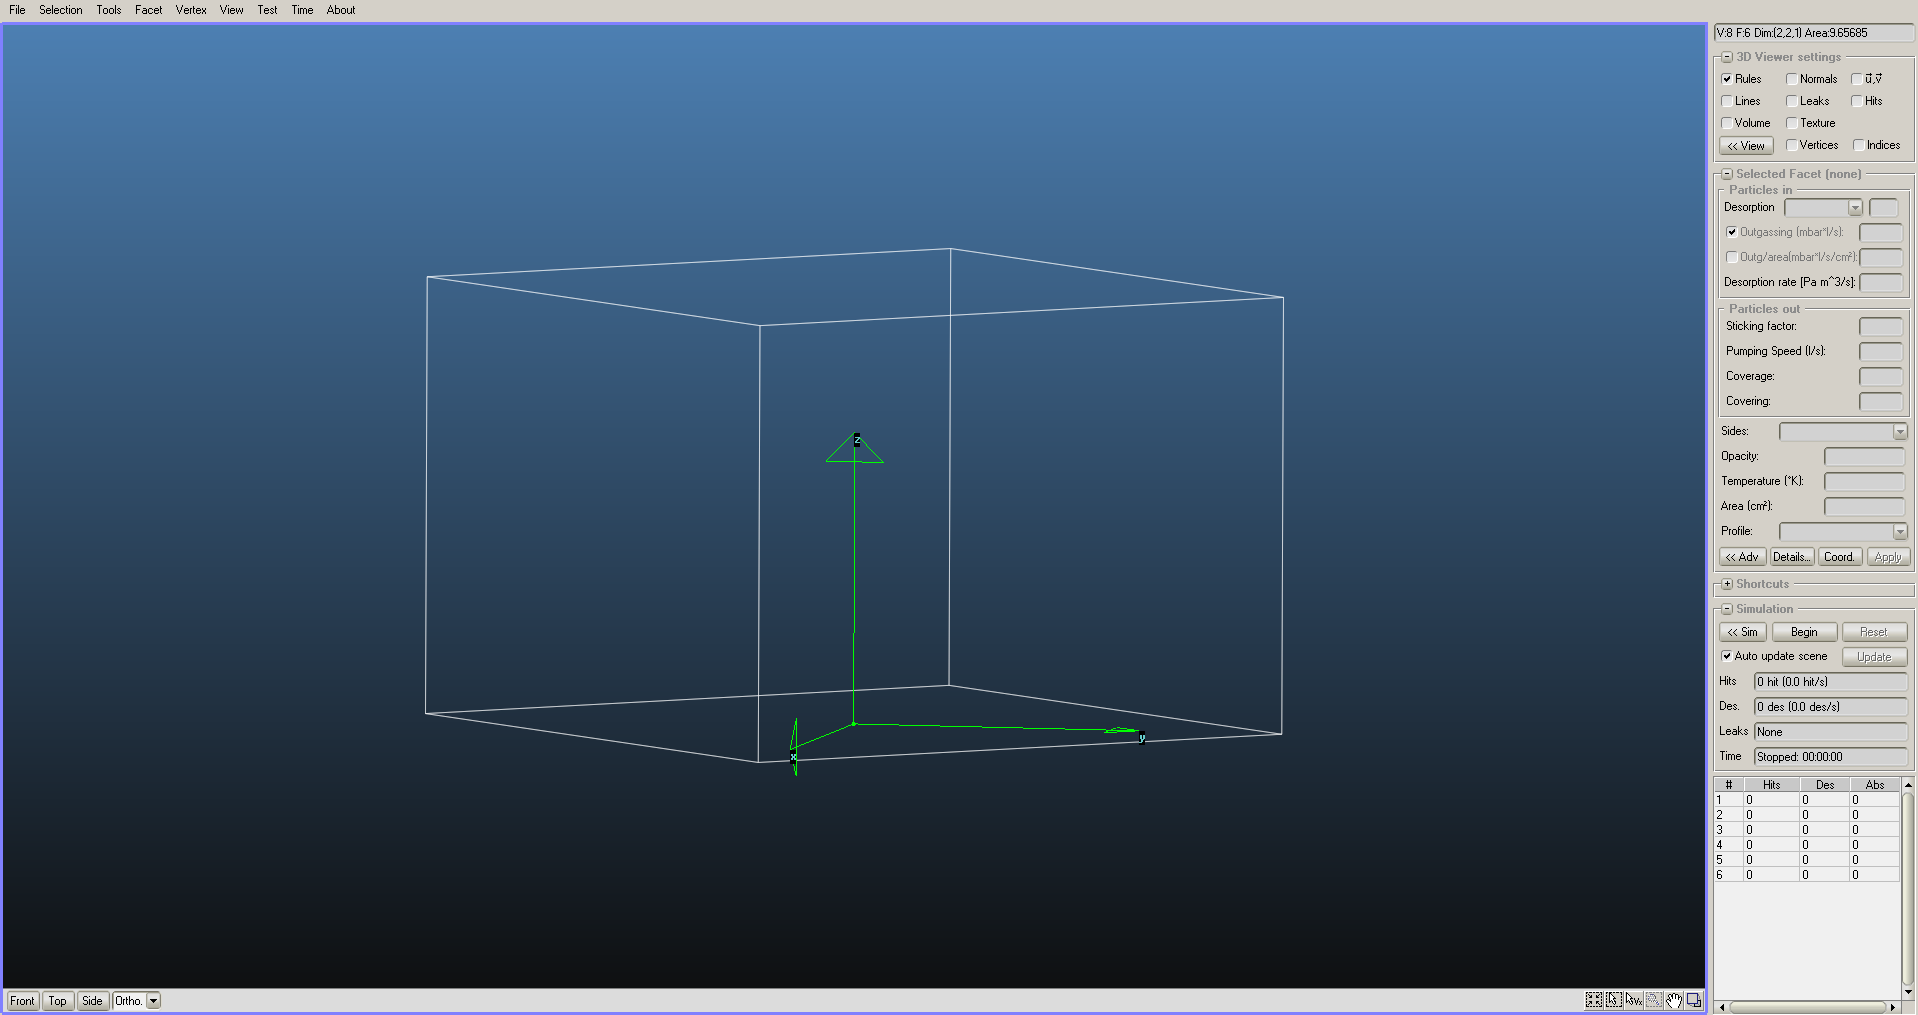
\includegraphics[width=\linewidth]{figures/ContWin}
\end{figure}

\subsubsection{New GUI elements}
\begin{itemize}[noitemsep,topsep=0pt]
\item "Particles out" %renamed to Contamination level
\begin{itemize}[noitemsep,topsep=0pt]
\item Text field for covering
\item Text field for coverage
\end{itemize}
%\item New facet properties
%\begin{itemize}[noitemsep,topsep=0pt]
%\item Effective surface factor
%\item Facet depth and facet volume
%\item Diffusion coefficient
%\item Concentration and gas mass
%\end{itemize}
%\item Text field for new sticking coefficient
%\item Window for CoveringHistory (reworked to SimulationHistory in ContaminationFlow Linux)
%\item PressureEvolution window expanded
%	\begin{itemize}[noitemsep,topsep=0pt]
%	\item Added list that contains information of graph
%	\item Option to show only selected facets or all
%	\item List exportable
%	\end{itemize}
\item New menu options
\begin{itemize}[noitemsep,topsep=0pt]
\item File: Export buffer, Export Cov.% Import buffer, Export Cov.
\item Selection: Export Selections
\end{itemize}
\end{itemize}

%\section{Application}
\section{Communication}
\subsubsection{Import and export of buffer files via GUI}
\begin{itemize}[noitemsep,topsep=0pt]
\item New Databuff struct \code{typedef unsigned char BYTE;\\typedef struct {\\
	\hphantom{\quad}signed int size;\\
	\hphantom{\quad}BYTE *buff;\\
}Databuff;}
\item New functions \codew{importBuff($\cdot$)} and \codew{exportBuff($\cdot$)} for import and export of buffer files/Databuff
\item New options in \codew{File} menu: \codew{Export buffer} and \codew{Import buffer}
\end{itemize}

\subsubsection{Export of Facet Groups}
\begin{itemize}[noitemsep,topsep=0pt]
\item New functions to output (text file or text field line) correct formating of facet groups for input file for ContaminationFlow Linux
\item New options in \codew{Selection} menu: \codew{Export Selections}
\end{itemize}

\subsubsection{Export of Covering/Coverage File}
\begin{itemize}[noitemsep,topsep=0pt]
\item Two output options: covering or coverage per facet
\item New functions to output (text file or text field line) correct formating of covering/coverage file for ContaminationFlow Linux
\item New options in \codew{File} menu: \codew{Export Cov.}
\end{itemize}


\section{New Quantities}
\subsubsection{New counter \codew{covering}}
\begin{itemize}[noitemsep,topsep=0pt]
\item Added covering counter to hitbuffer
\item Added covering to GUI, can be defined through textfield
\item Covering increased at adsorb
\end{itemize}
\begin{comment}

\subsubsection{New facet property \codew{effetiveSurfaceFactor}}
\begin{itemize}[noitemsep,topsep=0pt]
\item Defines increase of facet area due to texture
\end{itemize}


\subsubsection{New facet property \codew{facetDepth}}
\begin{itemize}[noitemsep,topsep=0pt]
\item Defines depth of facet
\end{itemize}


\subsubsection{New facet property \codew{diffusionCoefficient}}
\begin{itemize}[noitemsep,topsep=0pt]
\item Defines diffusion coefficient
\end{itemize}


\subsubsection{New facet property \codew{concentration}}
\begin{itemize}[noitemsep,topsep=0pt]
\item Defines concentration = mass of particles in volume
\end{itemize}

\subsubsection{Removal of irrelevant quantities}
\begin{itemize}[noitemsep,topsep=0pt]
\item Sticking factor and pumping speed removed from GUI
\item \codew{calcSticking()} and \codew{calcFlow()} in \codew{Molflow.cpp} file not used anymore
\item Flow not needed for iterative Algorithm
\end{itemize}

\end{comment}

%\section{Iterative algorithm}
%\subsubsection{New class to store covering for all facets at any time} 
%\begin{itemize}[noitemsep,topsep=0pt]
%\item In \codew{HistoryWin.cpp} and \codew{HistoryWin.h} file
%\item \codew{std::vector<std::pair<double,std::vector<double>\,>\,> pointintime\_list} to store points in time and respective covering for all facets
%\item New GUI option to add and remove entries for \codew{pointintime\_list}
%\item New GUI option to export or import a complete list
%\end{itemize}

%\section{Adaptation of Existing Code}
%\subsubsection{Thats changed}
%\begin{itemize}[noitemsep,topsep=0pt]
%\item use this for 
%\item list
%\end{itemize}
